\indent

% This section presents the high-level use case diagram of the system along with detailed visualizations of use cases. It provides a comprehensive view of system functionality, beginning with the big-picture interactions before focusing on specific use cases \textbf{under our responsibility}.
% \subsubsection{Overview diagram of usecases}
% \noindent
% \begin{minipage}{\textwidth}
%     \setlength{\parindent}{2em}
%     From the system requirements and user roles, we analyzed key interactions and designed an overview diagram of use cases to visualize the system's core functionalities. This diagram provides a clear, high-level overview of how users interact with the GMES system.
% \end{minipage}

% \begin{figure}[H]
%     \centering
%     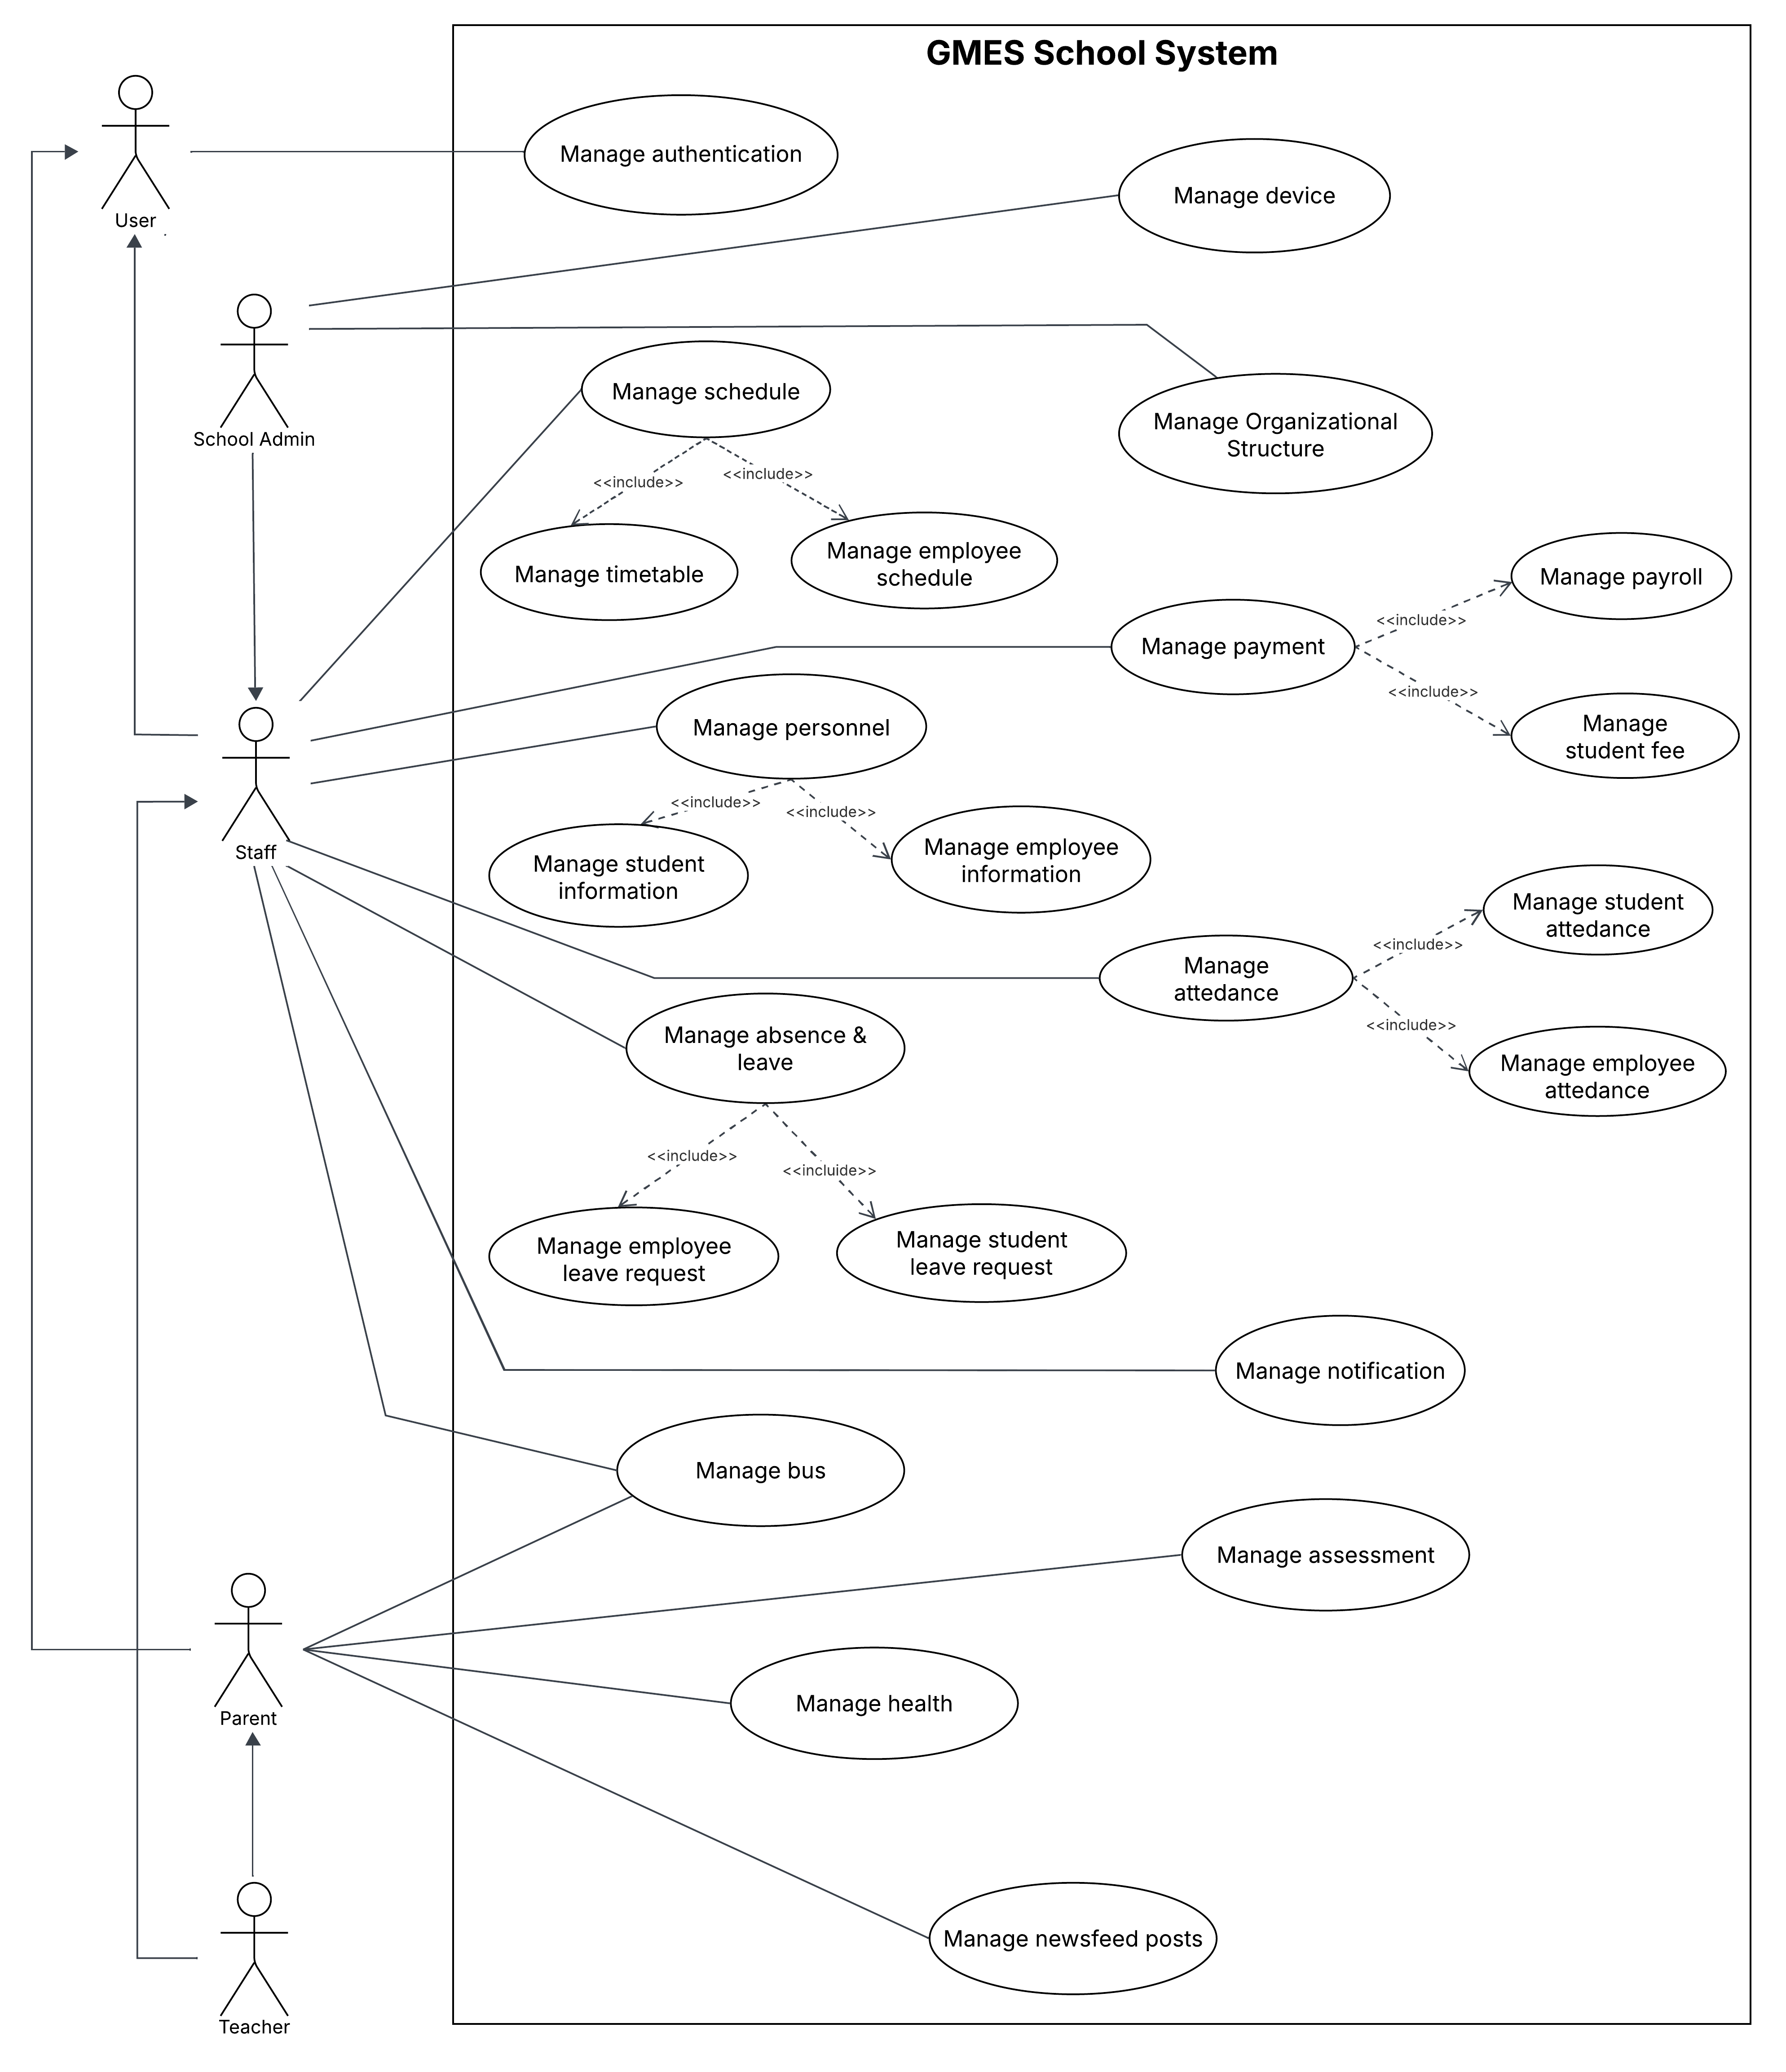
\includegraphics[width=1.1\linewidth]{images/use_case_diagram.png}
%     \vspace{-2.5em}
%     \caption{Overview diagram of use cases.}
%     \label{fig:overview_diagram_of_usecases}
% \end{figure}

\subsubsection{Detailed Use Case Diagrams}
\noindent
\begin{minipage}{\textwidth}
    \setlength{\parindent}{2em}
    While the previous section provided an overview of the system's functionalities, \textbf{this section presents detailed use case diagrams for each function under our responsibility} within the GMES School system. These diagrams illustrate the specific interactions between user roles and system features.
\end{minipage}
\vspace{0.5em}

% % AUTHENTICATION
% \indent\indent\textbf{2.4.2.1 Authentication usecase diagram}
% \vspace{0.5em}
% \par\indent\indent\parbox{0.9\textwidth}{
%     The Authentication function allow all users which use the GMES School system to securely access or exit the system.
% }
% \begin{figure}[H]
%     \centering
%     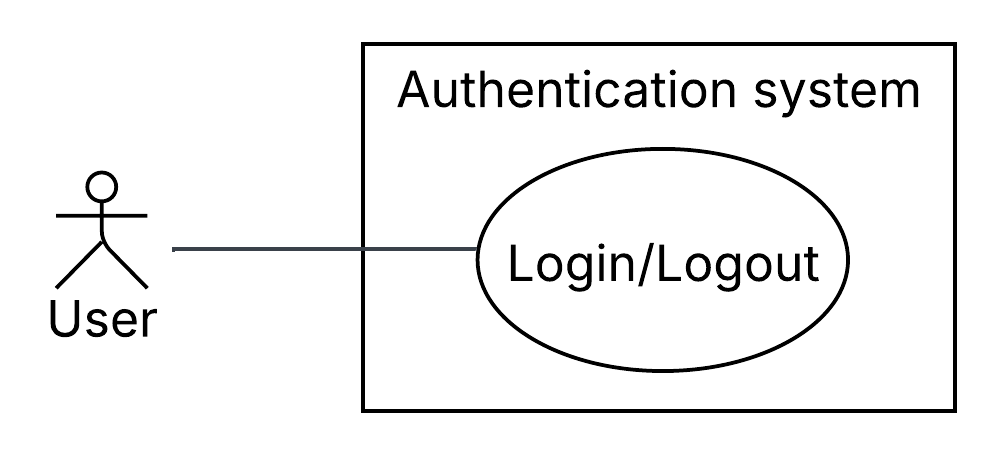
\includegraphics[width=0.6\textwidth]{images/use_case_login_logout.png}
%     \caption{Usecase diagram for login/logout.}
%     \label{fig:use_case_login_logout}
% \end{figure}

% PERSONNEL MANAGEMENT
% \newpage
% \indent\indent\textbf{2.4.2.1 Personnel Management Use Case Diagram}
% \vspace{0.5em}
% \par\indent\indent\parbox{0.9\textwidth}{
%     \setlength{\parindent}{2em}The Personnel Management module allows staff, school administrators, and teachers to manage personnel information. Staff and school administrators can manage employees, and students under their supervision, while teachers can only manage students under their supervision. This role-based approach prevents unauthorized access to sensitive information such as salary details, personal contracts, and student records, ensuring only authorized users can view or edit them. It also keeps information accurate by giving the right permissions to the right people.
% }\\
% \begin{figure}[H]
%     \centering
%     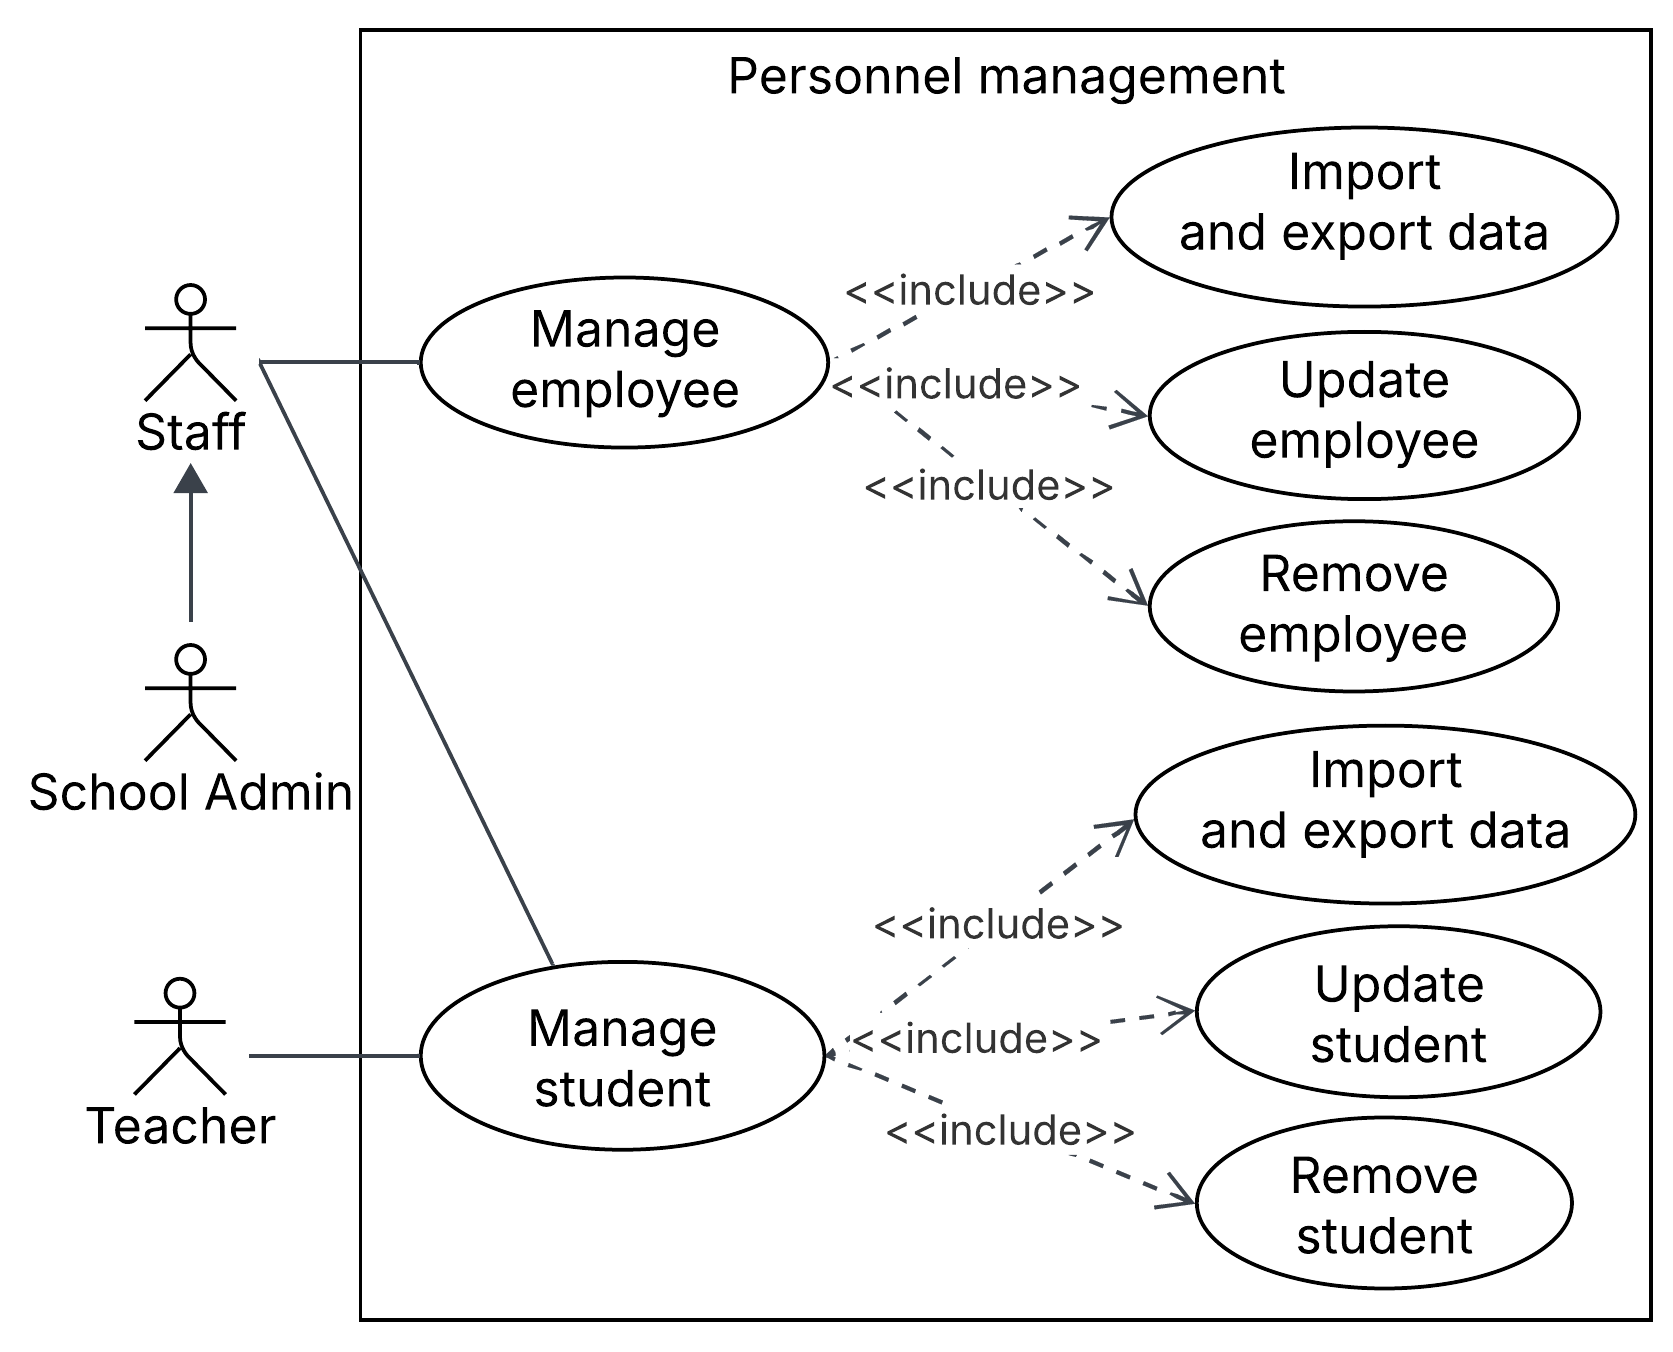
\includegraphics[width=0.7\textwidth]{images/use_case_personnel_management.png}
%     \caption{Use case diagram for Personnel Management.}
%     \label{fig:use_case_personnel_management}
% \end{figure}

% PERSONNEL MANAGEMENT: IMPORT EMPLOYEE DATA
% \renewcommand{\arraystretch}{1.5}
% \begin{longtable}{|>{\raggedright\arraybackslash}p{3.5cm}|
%                   >{\raggedright\arraybackslash}p{10cm}|}
% \caption{Import employee data via Excel basic flow.}
% \label{tab:employee_management_basic_flow} \\
% \endfirsthead
% \endhead
% \hline
%     \textbf{Function name} & \textbf{Import employee data}\\
%     \hline
%     Actor & Administrators and staff \\
%     \hline
%     Description & Support administrators and staff to import employee data to the database via Excel file \\
%     \hline
%     Pre-conditions & {
%         \vspace{-1.7em}
%         \begin{itemize}
%             \item The administrators and staff must log into the system with valid access rights
%             \vspace{-0.8em}
%             \item The uploaded file must be Excel file (.xlsx/.xls).
%             \vspace{-1.5em}
%         \end{itemize}    
%     }\\
%     \hline
%     Main flow &  {
%         \vspace{-1.7em}
%         \begin{itemize}
%             \item The administrators and staff access the Employee profiles feature.
%             \vspace{-0.8em}
%             \item The system gets the departments which are managed by the user (displayed in a tree structures).
%             \vspace{-0.8em}
%             \item Users select a department and uploaded the Excel file.
%             \vspace{-0.8em}
%             \item System validate the data in the uploaded file and save it to database.
%             \vspace{-0.8em}
%             \item Finish the process of importing employees data.
%             \vspace{-1.8em}
%         \end{itemize}    
%     }\\
%     \hline
% \end{longtable}

% ATTENDANCE MANAGEMENT
% \indent\indent\textbf{2.4.2.2 Attendance Management Use Case Diagram}
% \vspace{0.5em}
% \begin{adjustwidth}{3em}{0em}
%     \setlength{\parindent}{2em}
%     \leavevmode\indent
%     The Attendance Management module allows staff and school administrators to manage the attendance records of employees under their supervision, while teachers and school administrators can manage the attendance records of students under their supervision. Additionally, a parent can also view the attendance records of their child. For employees, attendance data is automatically recorded by timekeeping devices or it can be updated by the administrators and stored in the database. For students, attendance data is stored when the teacher marks the presence in class. This module will help organizations track the check-in/check-out time of employees to calculate their salary. It also improves communication between teacher and parent by sending notifications when teachers mark student attendance, giving parents better oversight of their child.
% \end{adjustwidth}    
% \begin{figure}[H]
%     \centering
%     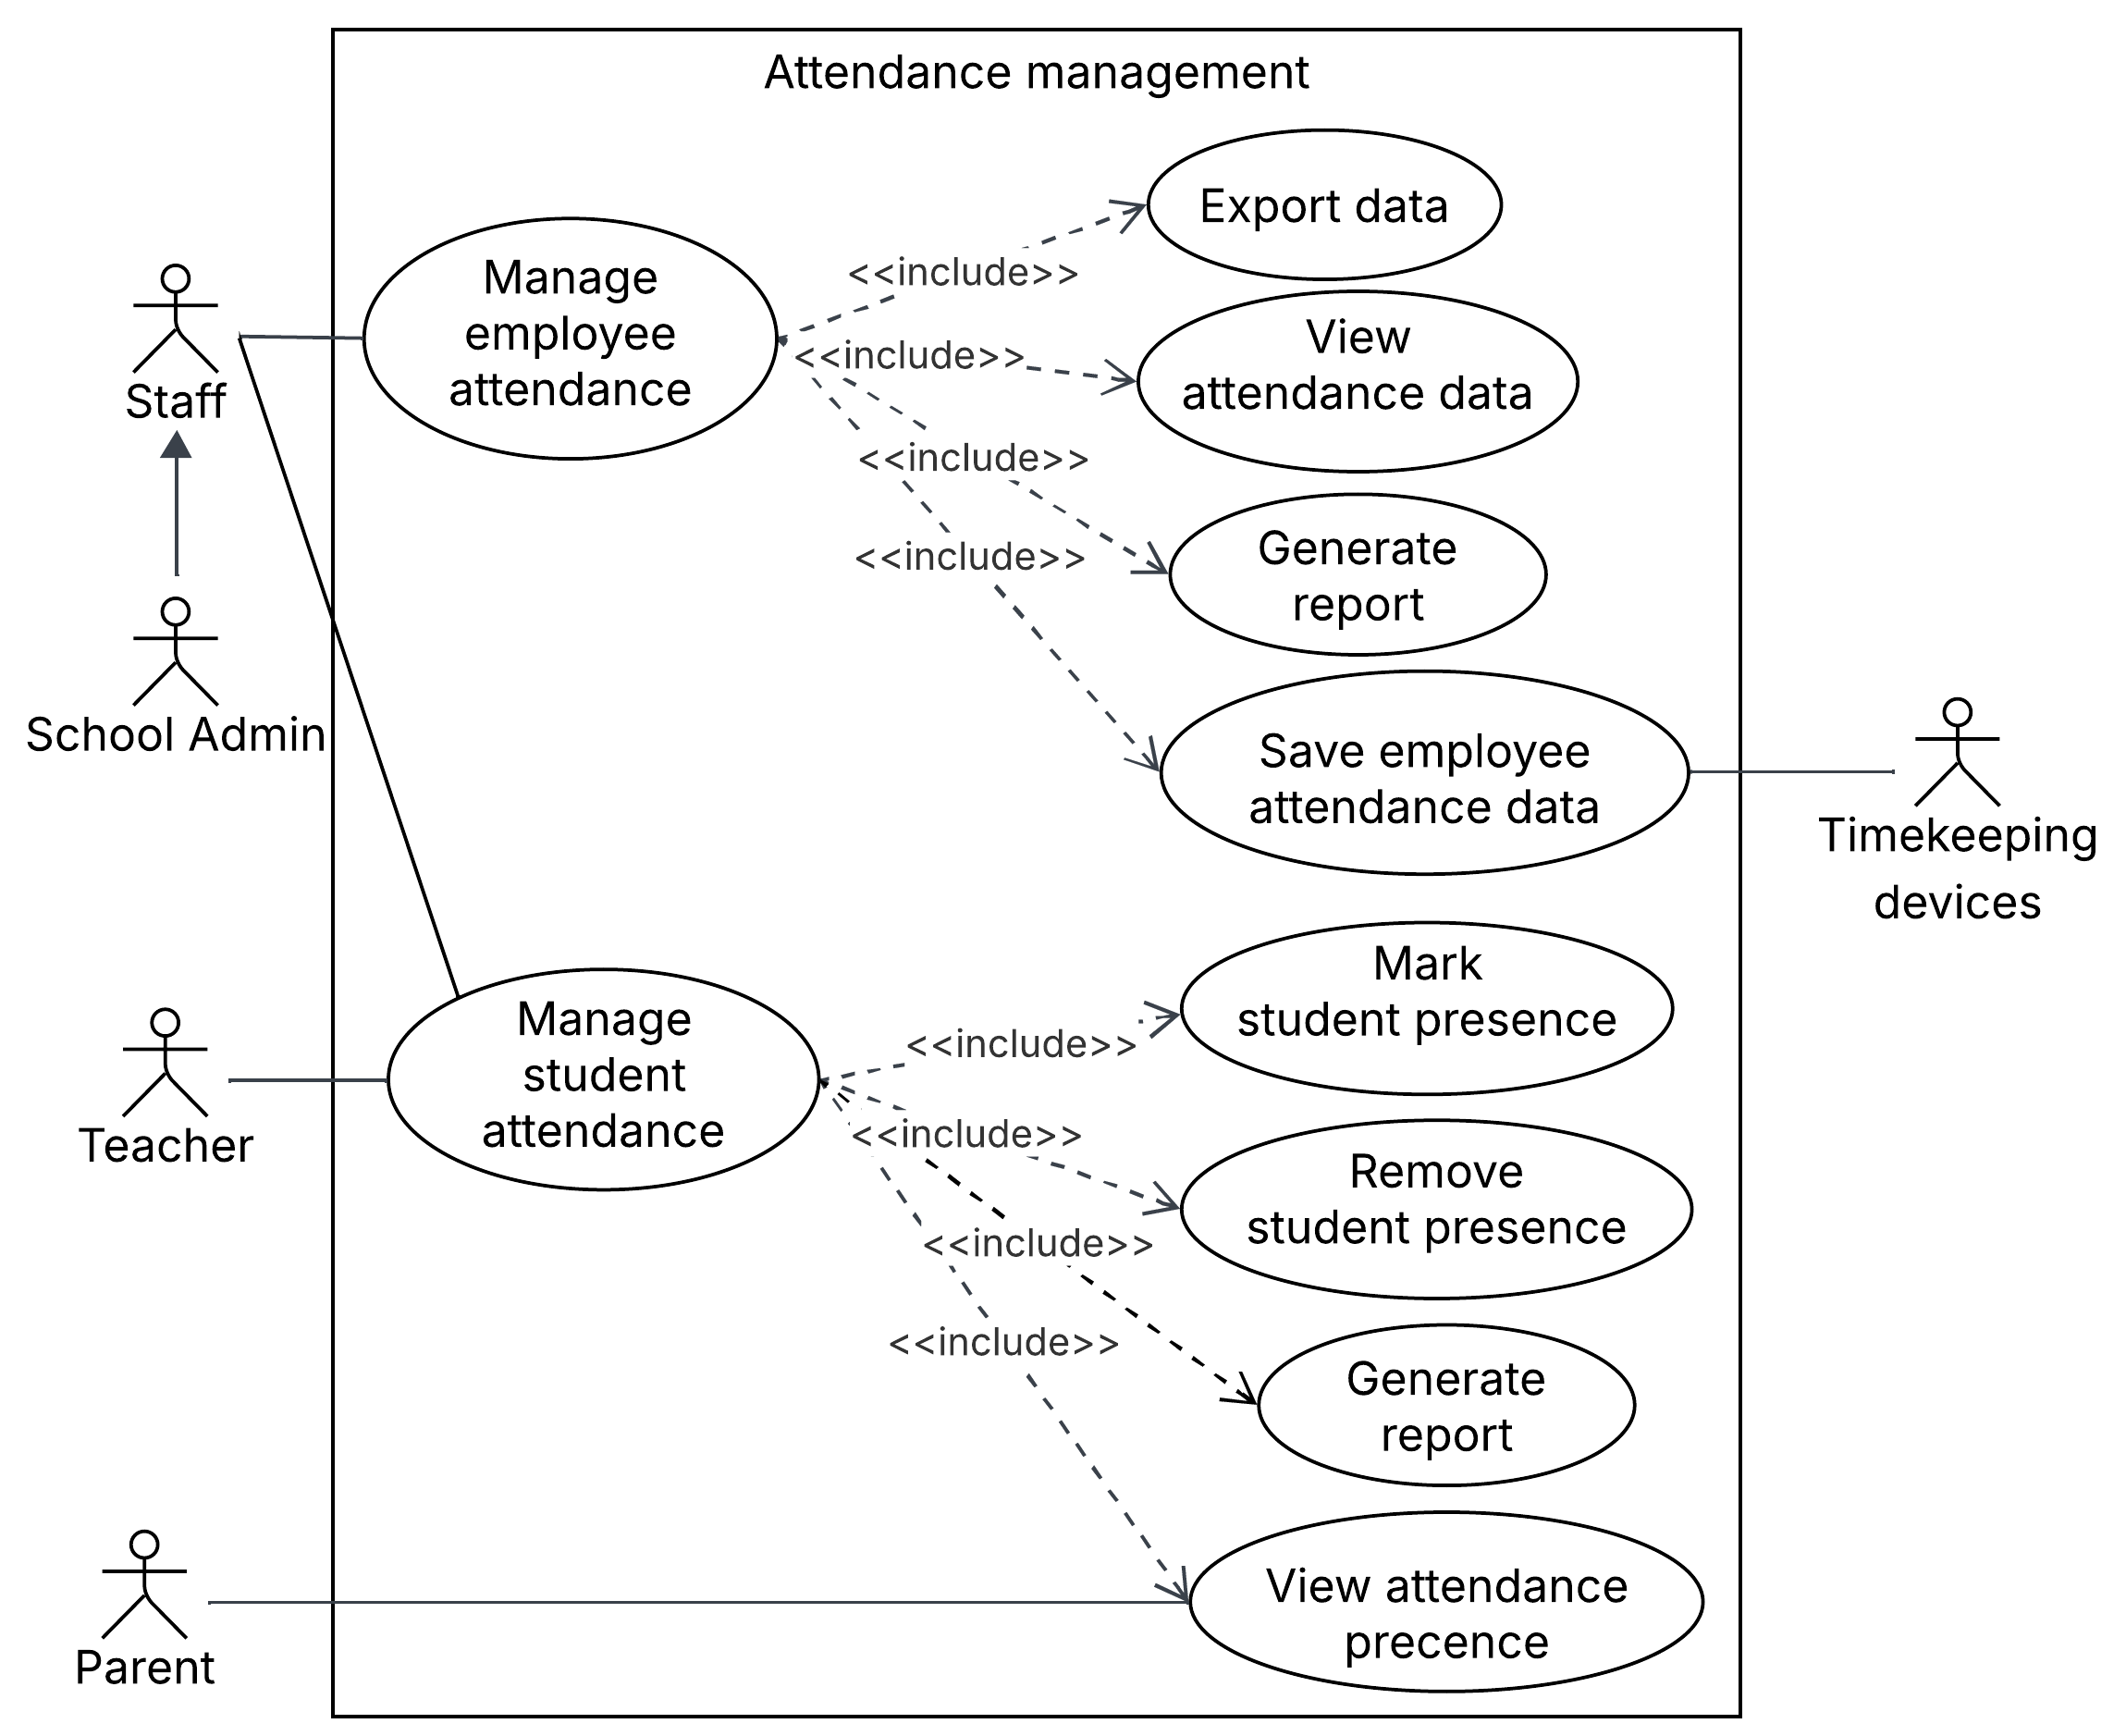
\includegraphics[width=\textwidth]{images/use_case_attendance_management.png}
%     \caption{Use case diagram for Attendance Management.}
%     \label{fig:use_case_attendance_management}
% \end{figure}

% ATTENDANCE MANAGEMENT: MARK ATTENDANCE IN CLASS
% \renewcommand{\arraystretch}{1.5}
% \begin{longtable}{|>{\raggedright\arraybackslash}p{3.5cm}|
%                   >{\raggedright\arraybackslash}p{10cm}|}
% \caption{Use Case Analysis for the Student Attendance Feature in Class.}
% \label{tab:attendance_management_student_attendance} \\
% \endfirsthead
% \endhead
% \hline
%     \textbf{Function name} & \textbf{Mark student attendance in class}\\
%     \hline
%     Actor & Teachers \\
%     \hline
%     Description & Support teachers to record student attendance when students arrive at class and when they leave to go home. \\
%     \hline
%     Pre-conditions & {
%         \vspace{-1.7em}
%         \begin{itemize}
%             \item The administrators and teachers must log into the system with valid access rights
%             \vspace{-0.8em}
%             \item The teachers must manage at least one class.
%             \vspace{-1.5em}
%         \end{itemize}    
%     }\\
%     \hline
%     Main flow &  {
%         \vspace{-1.7em}
%         \begin{itemize}
%             \item Teachers selects a class and access the Attendance feature
%             \vspace{-0.8em}
%             \item The system retrieves a list of students with their current status (checked/unchecked).
%             \vspace{-0.8em}
%             \item Teacher selects student and mark attendance status.
%             \vspace{-0.8em}
%             \item System save the records and push notification to parents.
%             \vspace{-0.8em}
%             \item Finish the process of marking student attendance data.
%             \vspace{-1.8em}
%         \end{itemize}    
%     }\\
%     \hline
% \end{longtable}

% LEAVE REQUEST MANAGEMENT
% \indent\indent\textbf{2.4.2.3 Leave Request Management Use Case Diagram}
% \vspace{0.5em}
% \begin{adjustwidth}{3em}{0em}
%     \setlength{\parindent}{2em}
%     \leavevmode\indent 
%     The Leave Request Management module enables school administrators, staff, teachers and parents to create, update, delete, and view leave requests. Parents can only manage leave requests for their own children, while teachers can manage their own requests and have the ability to review and confirm leave requests for students under their supervision. Staff and school administrators can manage leave requests for employees they supervise, including actions such as approving, declining, or canceling confirmed leave requests. Additionally, they can also export the leave request data of employees under their supervision to an Excel file. This module will reduce paperwork and manual errors in tracking absences. It also provides a clear working flow for requesting, reviewing, and approving or declining leave requests.
% \end{adjustwidth}   
% \begin{figure}[H]
%     \centering
%     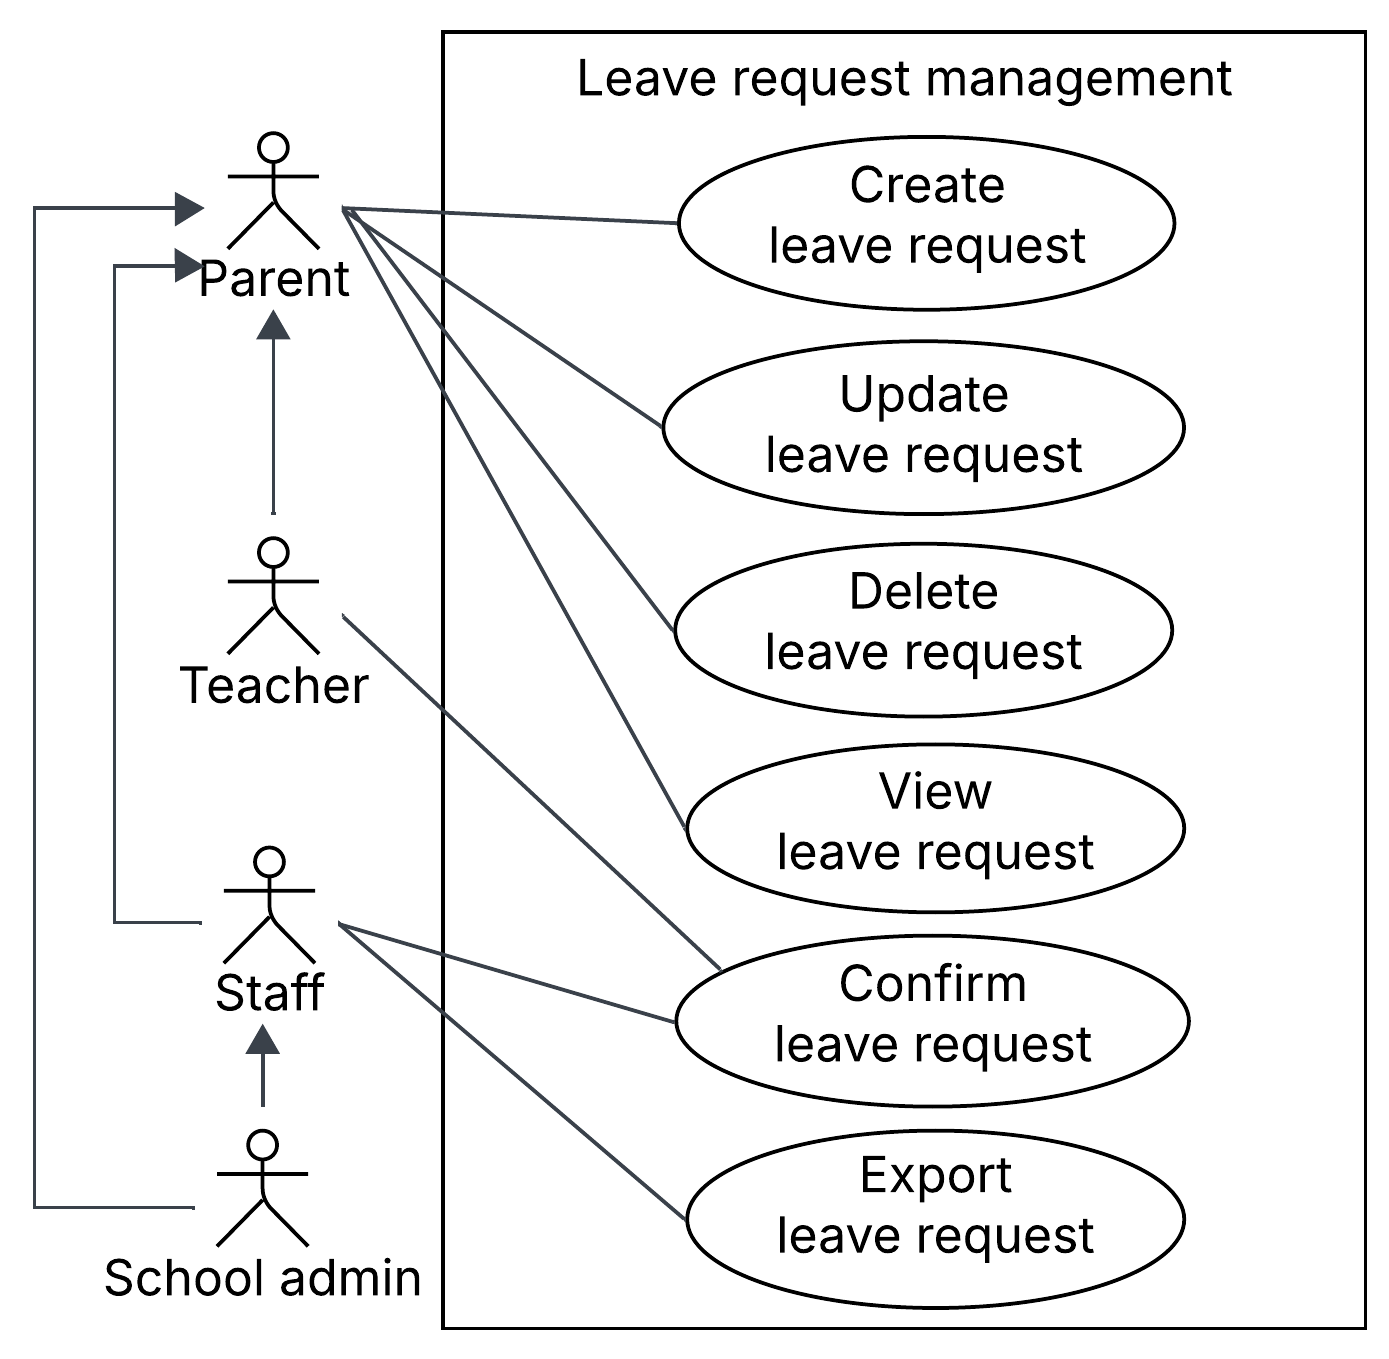
\includegraphics[width=0.55\textwidth]{images/use_case_leave_request_management.png}
%     \caption{Use case diagram for Leave Request Management.}
%     \label{fig:use_case_leave_request_management}
% \end{figure}

% LEAVE REQUEST MANAGEMENT: CREATE STUDENT LEAVE REQUEST
% \renewcommand{\arraystretch}{1.5}
% \begin{longtable}{|>{\raggedright\arraybackslash}p{3.5cm}|
%                   >{\raggedright\arraybackslash}p{10cm}|}
% \caption{Use Case Analysis for the Create Student Leave Request feature.}
% \label{tab:leave_management_student_leave_request} \\
% \endfirsthead
% \endhead
% \hline
%     \textbf{Function name} & \textbf{Create student leave request}\\
%     \hline
%     Actor & Parents \\
%     \hline
%     Description & Support parent create leave requests for their children \\
%     \hline
%     Pre-conditions & {
%         \vspace{-1.7em}
%         \begin{itemize}
%             \item The administrators and teachers must log into the system with valid access rights
%             \vspace{-0.8em}
%             \item The teachers must manage at least one class.
%             \vspace{-1.5em}
%         \end{itemize}    
%     }\\
%     \hline
%     Main flow &  {
%         \vspace{-1.7em}
%         \begin{itemize}
%             \item Teachers selects a class and access the Attendance feature
%             \vspace{-0.8em}
%             \item The system retrieves a list of students with their current status (checked/unchecked).
%             \vspace{-0.8em}
%             \item Teacher selects student and mark attendance status.
%             \vspace{-0.8em}
%             \item System save the records and push notification to parents.
%             \vspace{-0.8em}
%             \item Finish the process of marking student attendance data.
%             \vspace{-1.8em}
%         \end{itemize}    
%     }\\
%     \hline
% \end{longtable}
    


% NEWSFEED MANAGEMENT
% \indent\indent\textbf{2.4.2.4 Newsfeed management Use Case Diagram}
% \vspace{0.5em}
% \par\indent\indent\parbox{0.9\textwidth}{
%     \setlength{\parindent}{2em} 
%     The Newsfeed Management is a communication module that allows teachers to share classroom and school activities through images, videos, and files. Teachers can create, edit, view, comment on, react to, and delete content for the classes they supervise, while parents can only view, comment on, and react to these posts. This feature provides parents with valuable insights into their child's class experiences and improves the connection between home and school.
% }\\
% \begin{figure}[H]
%     \centering
%     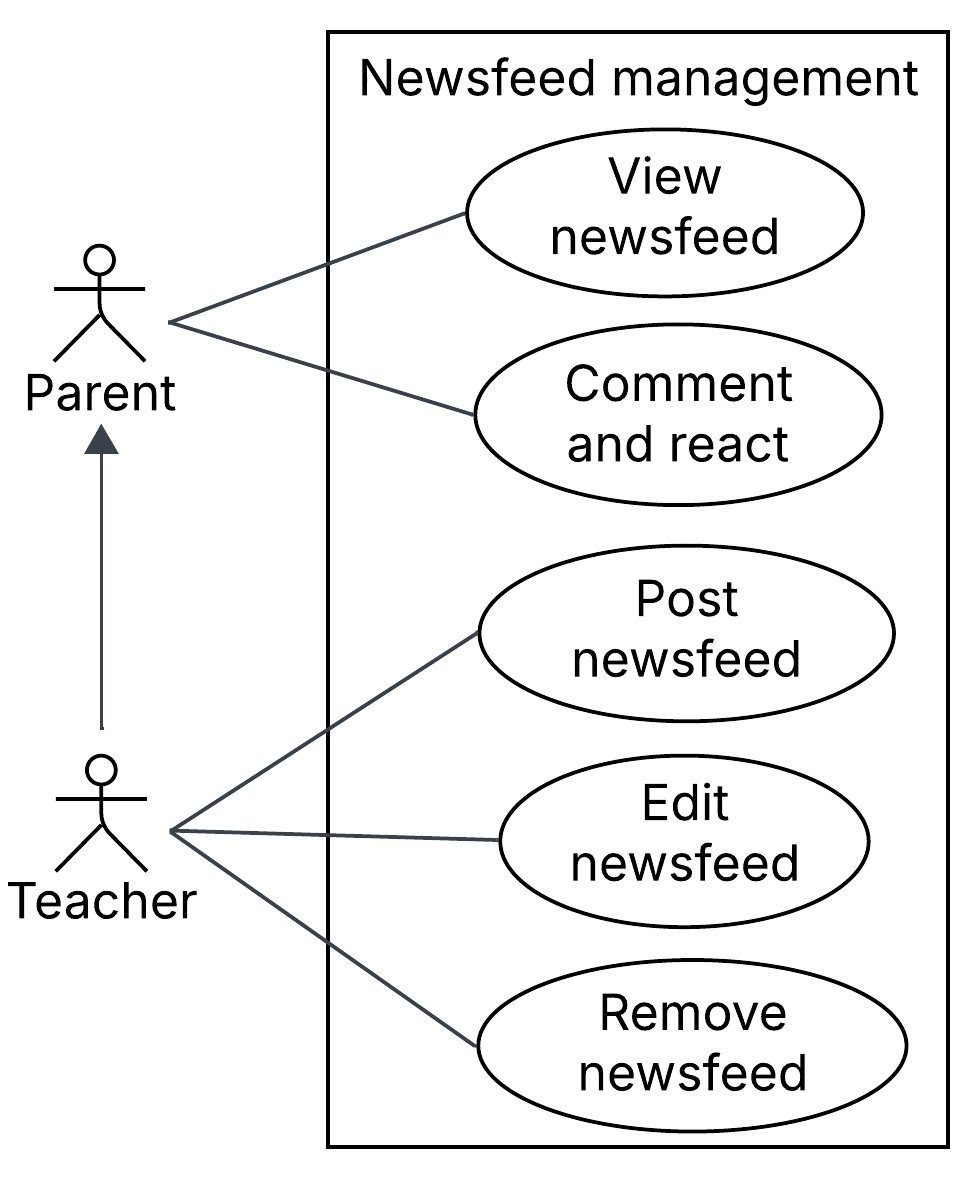
\includegraphics[width=0.5\textwidth]{images/use_case_newsfeed_management.png}
%     \vspace{-0.5em}
%     \caption{Use case diagram for Newsfeed Management.}
%     \label{fig:use_case_newsfeed_management}
% \end{figure}
    

% STUDENT ASSESSMENT MANAGEMENT
% \indent\indent\textbf{2.4.2.5 Student Assessment Management Use Case Diagram}
% \vspace{0.5em}
% \par\indent\indent\parbox{0.9\textwidth}{
%     \setlength{\parindent}{2em} 
%     Student Assessment Management is a module that allows teachers to evaluate individual or multiple students. Teachers can create, modify, and view assessments for the students they supervise, while parents can only view assessments of their children. Additionally, teachers can add supporting files such as images or files for assessment to make it more reliable. This feature helps parent tracks their child's academic progress, achievements, and overall performance in the class.
% }\\
% \begin{figure}[H]
%     \centering
%     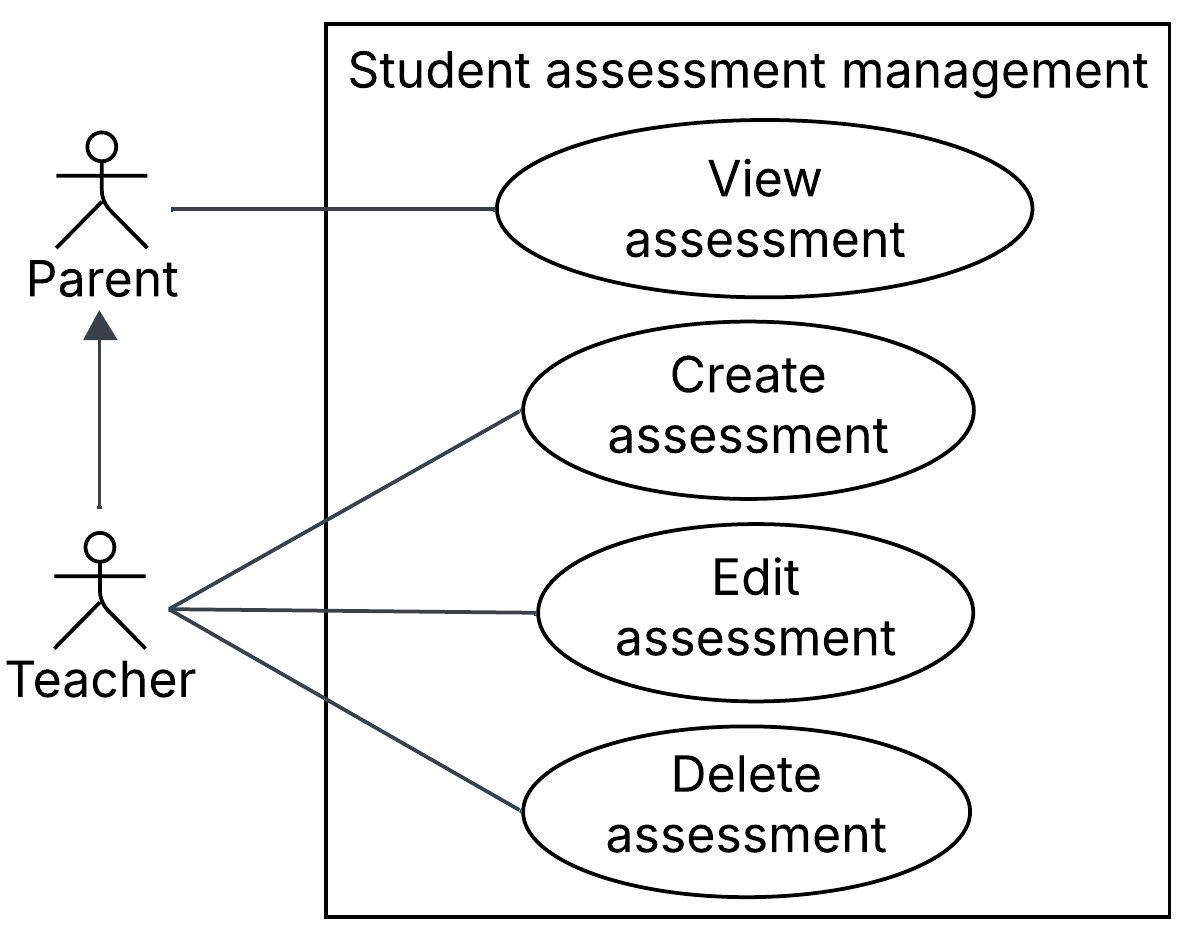
\includegraphics[width=0.6\textwidth]{images/use_case_student_assessment_management.png}
%     \caption{Use case diagram for Student Assessment Management.}
%     \label{fig:use_case_student_assessment_management}
% \end{figure}

% MEDICINE REMINDER MANAGEMENT
% \indent\indent\textbf{2.4.2.6 Medicine Reminder Management Use Case Diagram}
% \vspace{0.5em}
% \par\indent\indent\parbox{0.9\textwidth}{
%     \setlength{\parindent}{2em}
%     Medicine Reminder Management is a module that allows parents to remind teachers to administer medication to their children. Parents can create, modify, delete, and view medicine reminders for their children, while teachers can only view and confirm these reminders. Once a medicine reminder is confirmed by a teacher, parents cannot modify or delete it to ensure accountability and prevent confusion. Additionally, parents can attach images to the reminders to increase reliability. This feature helps ensure proper medication administration while maintaining clear communication between parents and teachers, ultimately supporting children's health and safety in the educational environment.
% }\\
% \begin{figure}[H]
%     \centering
%     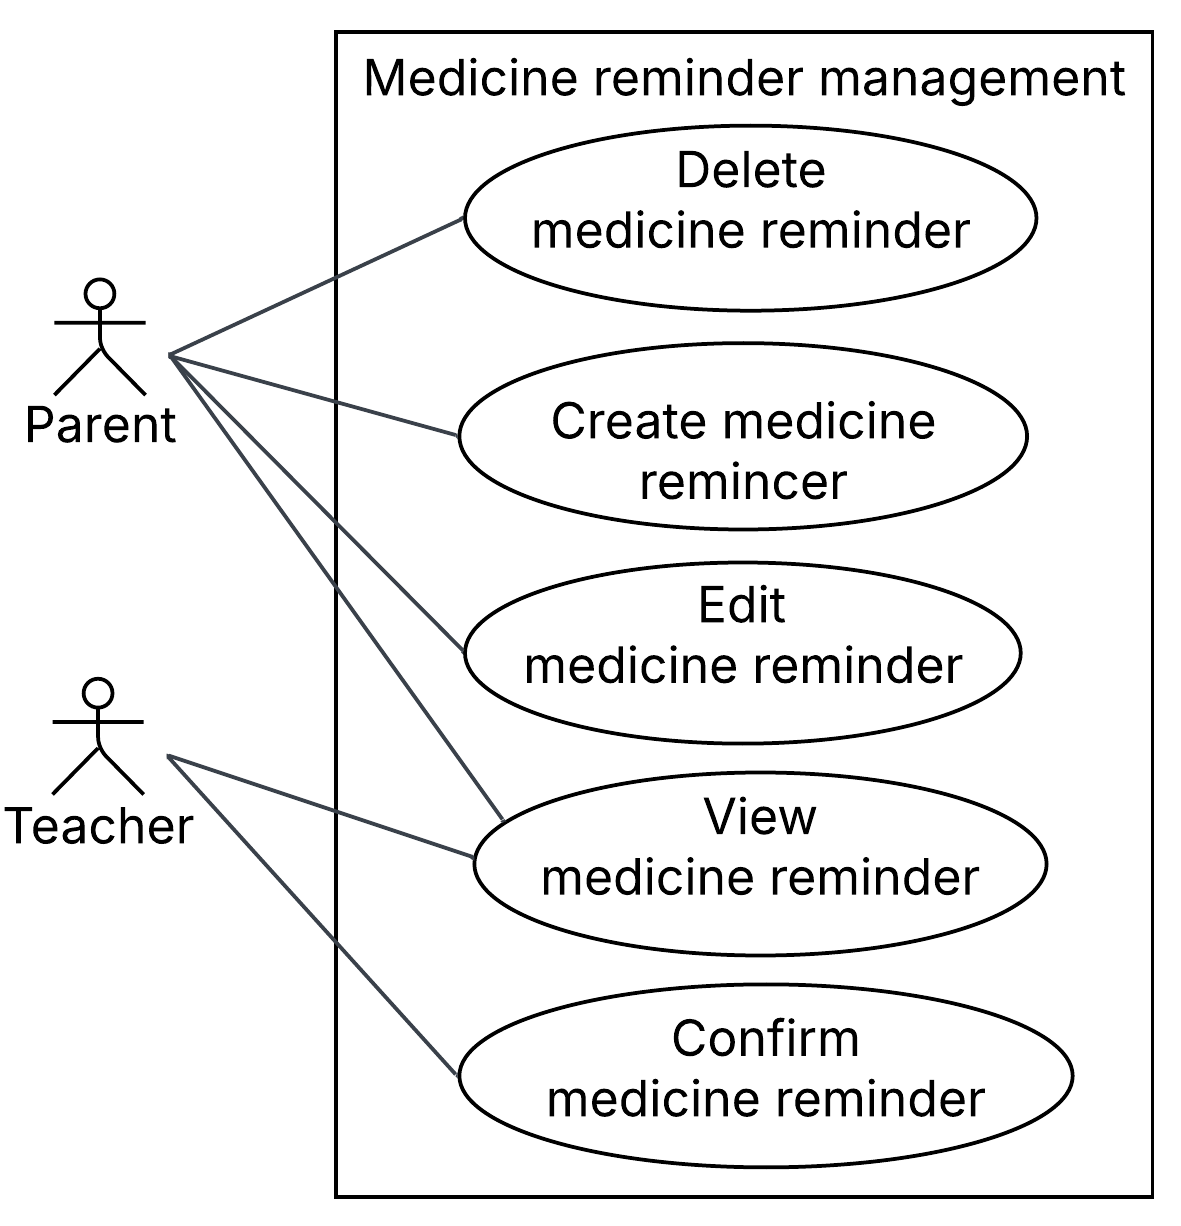
\includegraphics[width=0.55\textwidth]{images/use_case_medicine_reminder.png}
%     \caption{Use case diagram for Medicine Reminder Management.}
%     \label{fig:use_case_medicine_reminder_management}
% \end{figure}

% NOTIFICATION MANAGEMENT
% \indent\indent\textbf{2.4.2.7 Notification Management Use Case Diagram}
% \vspace{0.5em}
% \par\indent\indent\parbox{0.9\textwidth}{
%     \setlength{\parindent}{2em}
%     Notification Management is a module that serves as a communication bridge between schools and parents. School administrators and teachers can create, edit, delete, push, and view notifications, while parents can only receive and read all notifications sent by the school. This feature ensures parents stay informed about important school updates, events, and announcements. The notifications will be pushed to the parent mobile device, and this module eliminates the need for paper notices or phone calls.
% }\\
% \begin{figure}[H]
%     \centering
%     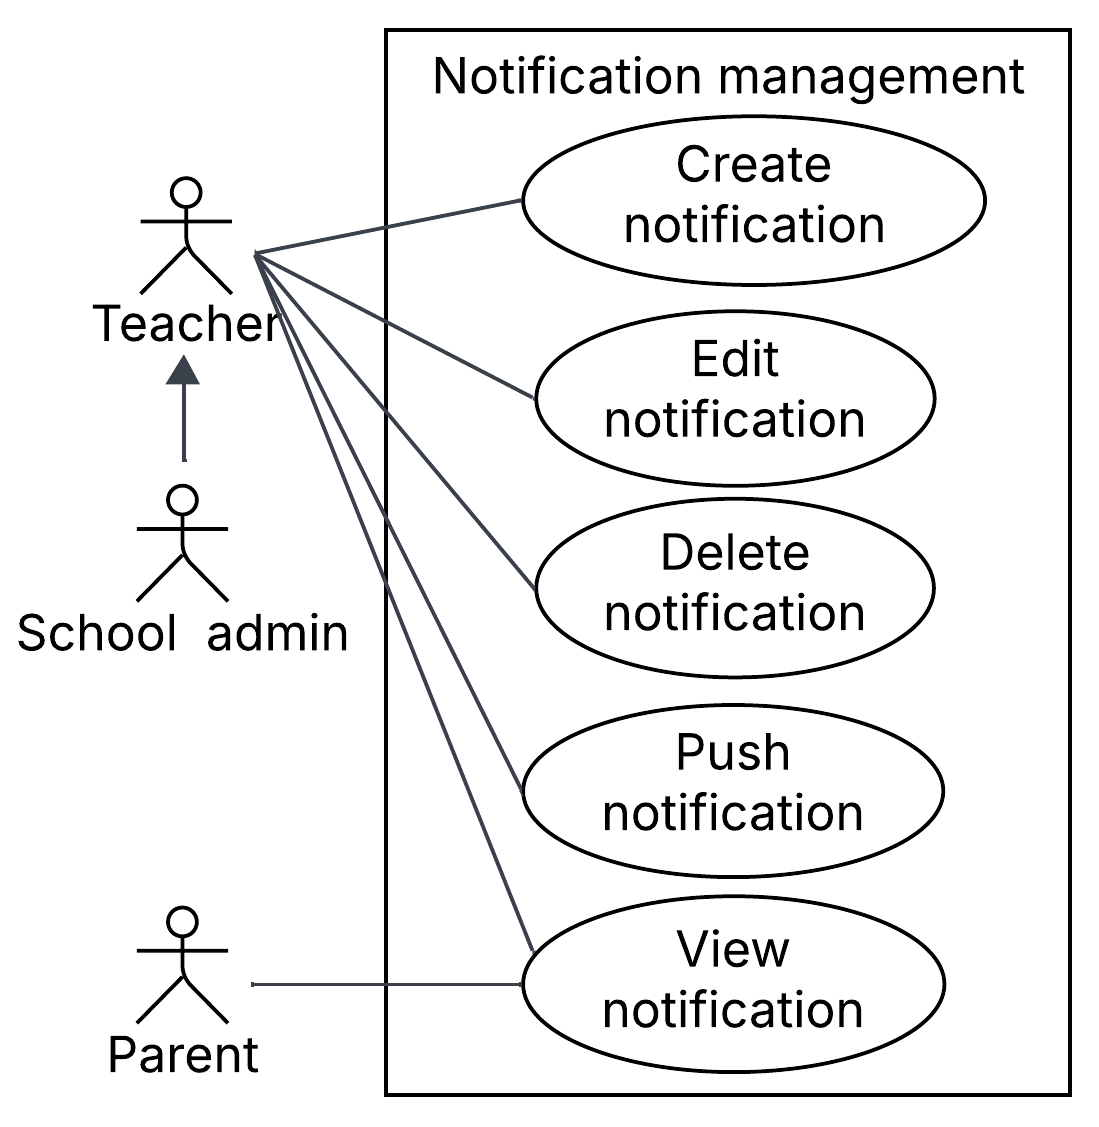
\includegraphics[width=0.55\textwidth]{images/use_case_notification_management.png}
%     \caption{Use Case diagram for Notification Management.}
%     \label{fig:use_case_notification_management}
% \end{figure}

% BUS MANAGEMENT
% \newpage
% \indent\indent\textbf{2.4.2.8 Bus Management Use Case Diagram}
% \vspace{0.5em}
% \par\indent\indent\parbox{0.9\textwidth}{
%     \setlength{\parindent}{2em}
%     Bus Management is a module that manages all aspects related to school transportation services within educational institutions. It enables administrators and staff to efficiently configure, view, and delete bus routes as well as register bus stops for students, ensuring optimized resource allocation and reduced manual time. For parents, the module provides real-time bus tracking and the ability to register designated stops, along with access to bus route information for their children, enhancing transparency and safety.
% }\\
% \begin{figure}[H]
%     \centering
%     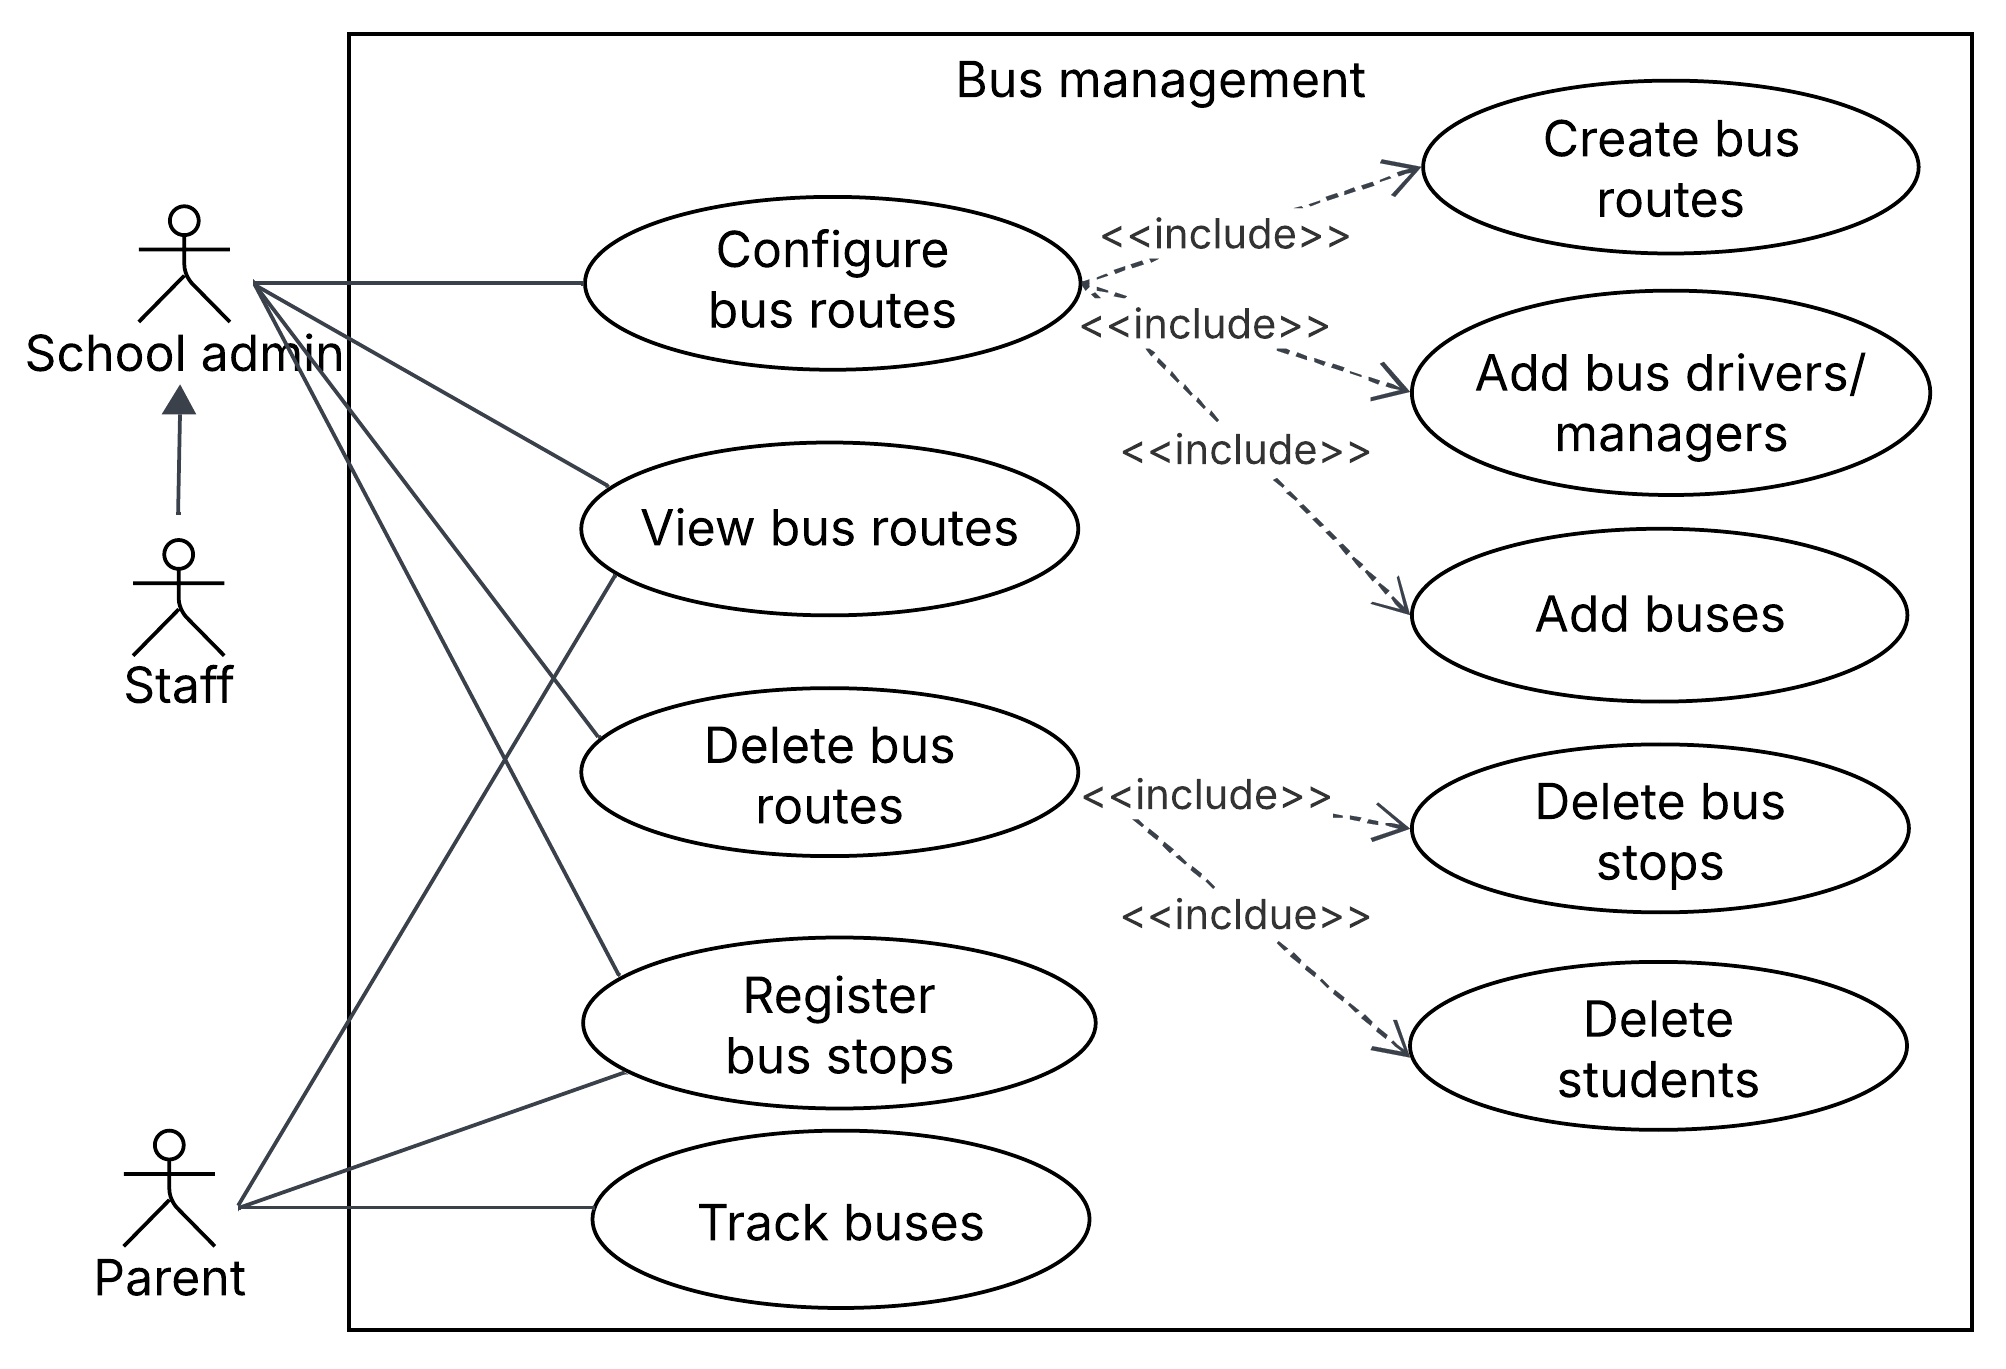
\includegraphics[width=0.9\textwidth]{images/use_case_bus_management.png}
%     \caption{Use Case diagram for Bus Management.}
%     \label{fig:use_case_bus_management}
% \end{figure}
